\section{Visual Design} % or "Research Plan"
\label{sec:vis}

Our ultimate goal, is to design a visualization tool for understanding courses interactions. Our target users are professors, students and academic advisors. We talk with graduate students and professors about what they need to summarize our tasks as below:
\begin{itemize}
	\item [T1] Overview of clusters of correlated courses
	\item [T2] For a specific course, find the courses which potentially benefit it and compare the importance of these courses
	\item [T3] For two selected courses, show details of student grades
\end{itemize}

We preprocess our original data and choose to use all the course records of computer science department for our implementations. We carefully select the visualization techniques which can be easily understood by users. Our system has three major view: the adjacency matrix, bar chart view and parallel coordinates view. In this section. We describe all the works we have done and the details of Coursim.~\ref{sec:background}.

%\You may want to use figures to illustrate your point, such as
%\Figure~\ref{fig:sample}.

\begin{figure}[h]
 \centering % avoid the use of \begin{center}...\end{center} and use \centering instead (more compact)
 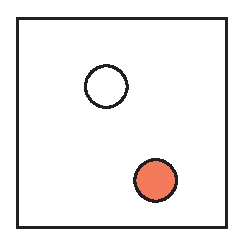
\includegraphics[width=\columnwidth]{figs/sample} 
 \caption{Figure illustrating some component of your design.}
 \label{fig:sample}
\end{figure}

%\begin{figure*}[h]
% \centering 
% 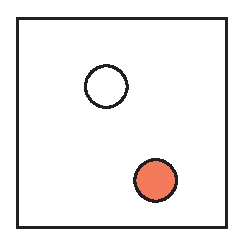
\includegraphics[width=\textwidth]{figs/sample} 
% \caption{Double Column Figure.}
% \label{fig:sample2}
%\end{figure*}

